\documentclass[../main.tex]{subfiles}

\graphicspath{{\subfix{../images/}}}

\begin{document}

\clearpage
\thispagestyle{empty}
\subsection{Esercitazione V}

La quinta esercitazione di Controlli Automatici è dedicata all’analisi e verifica delle prestazioni di sistemi lineari a tempo invariante (LTI) soggetti a retroazione, mediante l’utilizzo di un controllore statico a guadagno costante. Attraverso gli esercizi proposti, vengono affrontati e approfonditi i principali strumenti di analisi sia nel dominio della frequenza (diagrammi di Bode, Nyquist, verifica della stabilità tramite criteri grafici) che nel dominio del tempo, con particolare attenzione al calcolo dell’errore di inseguimento in regime permanente in presenza di differenti ingressi e disturbi.

L’esercitazione offre infine l’opportunità di collegare strettamente le analisi teoriche con la verifica sperimentale mediante simulazione.

\vspace*{1cm}
\subsubsection{Analisi della stabilità e del comportamento in regime permanente di un sistema retroazionato}
\label{lab51}

Sia dato il sistema LTI descritto dalla seguente funzione di trasferimento:

\begin{equation}
	F(s) = \frac{s^2 + 11s + 10}{s^4 + 4s^3 + 8s^2}
\end{equation}

controllato mediante un controllore statico di guadagno $K_c$ (da definire), chiuso in un anello di retroazione negativa con un blocco di guadagno $1/K_r$, secondo lo schema riportato in figura:

\begin{figure}[h!]
\begin{center}

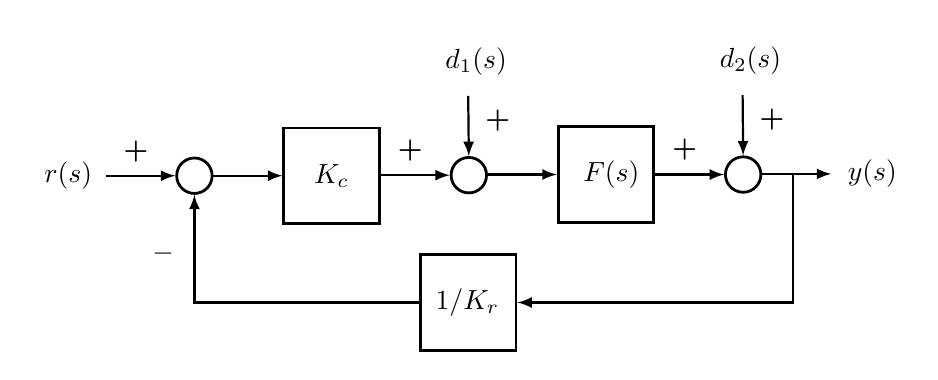
\begin{tikzpicture}[transform shape]
	\node[shape=rectangle, draw, line width=1pt, minimum width=1.215cm, minimum height=1.215cm] at (18.265, -14.015){};
	\draw[line width=0.8pt, -latex] (18.89, -14.008) -- (19.765, -14.008);
	\node[shape=circle, draw, line width=1pt, minimum width=0.45cm] at (20.008, -14.008){};
	\node[shape=circle, draw, line width=1pt, minimum width=0.45cm] at (16.523, -14.015){};
	\draw[line width=0.8pt, -latex] (15.405, -14.015) -- (16.28, -14.015);
	\draw[line width=0.8pt, -latex] (16.765, -14.015) -- (17.64, -14.015);
	\node[shape=rectangle, draw, line width=1pt, minimum width=1.215cm, minimum height=1.215cm] at (21.75, -14){};
	\draw[line width=0.8pt, -latex] (20.25, -14) -- (21.125, -14);
	\node[shape=rectangle, draw, line width=1pt, minimum width=1.215cm, minimum height=1.215cm] at (20, -15.625){};
	\draw[line width=0.8pt, -latex] (20, -13) -- (20.008, -13.765);
	\draw[line width=0.8pt, -latex] (19.375, -15.625) -| (16.523, -14.258);
	\node[shape=rectangle, minimum width=0.965cm, minimum height=0.84cm] at (14.905, -14.015){} node[anchor=center, align=center, text width=0.577cm, inner sep=6pt] at (14.905, -14.015){$r(s)$};
	\node[shape=rectangle, minimum width=0.965cm, minimum height=0.84cm] at (18.265, -14.015){} node[anchor=center, align=center, text width=0.577cm, inner sep=6pt] at (18.265, -14.015){$K_c$};
	\node[shape=rectangle, minimum width=0.965cm, minimum height=0.84cm] at (19.875, -15.625){} node[anchor=center, align=center, text width=0.577cm, inner sep=6pt] at (19.875, -15.625){$1/K_r$};
	\node[shape=rectangle, minimum width=0.965cm, minimum height=0.84cm] at (20, -12.562){} node[anchor=center, align=center, text width=0.577cm, inner sep=6pt] at (20, -12.562){$d_1(s)$};
	\node[shape=rectangle, minimum width=0.965cm, minimum height=0.84cm] at (21.75, -14){} node[anchor=center, align=center, text width=0.577cm, inner sep=6pt] at (21.75, -14){$F(s)$};
	\node[shape=rectangle, minimum width=0.965cm, minimum height=0.84cm] at (25.11, -13.992){} node[anchor=center, align=center, text width=0.577cm, inner sep=6pt] at (25.11, -13.992){$y(s)$};
	\draw[line width=0.8pt, -latex] (24.125, -14) |- (20.625, -15.625);
	\node[shape=rectangle, minimum width=0.715cm, minimum height=0.59cm] at (15.78, -13.703){} node[anchor=center, align=center, text width=0.327cm, inner sep=6pt] at (15.78, -13.703){$\textbf{+}$\\};
	\node[shape=rectangle, minimum width=0.715cm, minimum height=0.59cm] at (20.375, -13.313){} node[anchor=center, align=center, text width=0.327cm, inner sep=6pt] at (20.375, -13.313){$\textbf{+}$\\};
	\node[shape=rectangle, minimum width=0.715cm, minimum height=0.59cm] at (19.265, -13.695){} node[anchor=center, align=center, text width=0.327cm, inner sep=6pt] at (19.265, -13.695){$\textbf{+}$\\};
	\node[shape=rectangle, minimum width=0.715cm, minimum height=0.59cm] at (16.125, -15){} node[anchor=center, align=center, text width=0.327cm, inner sep=6pt] at (16.125, -15){$-$\\};
	\draw[line width=0.8pt, -latex] (22.375, -14) -- (23.25, -14);
	\node[shape=circle, draw, line width=1pt, minimum width=0.45cm] at (23.492, -14){};
	\draw[line width=0.8pt, -latex] (23.735, -13.992) -- (24.61, -13.992);
	\draw[line width=0.8pt, -latex] (23.485, -12.992) -- (23.492, -13.758);
	\node[shape=rectangle, minimum width=0.965cm, minimum height=0.84cm] at (23.485, -12.555){} node[anchor=center, align=center, text width=0.577cm, inner sep=6pt] at (23.485, -12.555){$d_2(s)$};
	\node[shape=rectangle, minimum width=0.715cm, minimum height=0.59cm] at (23.86, -13.305){} node[anchor=center, align=center, text width=0.327cm, inner sep=6pt] at (23.86, -13.305){$\textbf{+}$\\};
	\node[shape=rectangle, minimum width=0.715cm, minimum height=0.59cm] at (22.75, -13.688){} node[anchor=center, align=center, text width=0.327cm, inner sep=6pt] at (22.75, -13.688){$\textbf{+}$\\};
\end{tikzpicture}
	
	
\label{lab501}
\caption{Schema del sistema LTI preso in esame}	
\end{center}	
\end{figure}


Sia $G_a(s) \frac{K_c}{K_r}$ la funzione di trasferimento d’anello del sistema retroazionato, ove $K_r$ = 1.

\begin{enumerate}[label=\alph*]
	\item Determinare, con l’ausilio di \textsc{Matlab}, il guadagno stazionario $K_F$ della funzione $F(s)$ e le sue singolarità, evidenziandone parte reale e parte immaginaria, nonché pulsazione naturale e fattore di smorzamento per eventuali singolarità complesse coniugate. Calcolare quindi la fase iniziale (per $\omega \rightarrow 0^+$) e la fase finale (per $\omega \rightarrow +\infty$) di $F(j \omega)$.
	\item Dopo aver tracciato qualitativamente a mano i diagrammi di Bode di $G_a(j\omega)$ per $K_c$ = 1, determinarne l’andamento esatto con l’ausilio di \textsc{Matlab}.
	\item Tracciare qualitativamente il diagramma di Nyquist della funzione $G_a(j\omega)$ sopra definita e quotarne i principali punti di interesse (ovvero gli attraversamenti dell’asse reale) con l’ausilio di \textsc{Matlab}.
	\item Verificare la stabilità del sistema ad anello chiuso per $K_c$ = 1 mediante applicazione del criterio di Nyquist. Verificare inoltre la correttezza del risultato ottenuto mediante calcolo diretto dei poli della funzione di trasferimento ad anello chiuso $W(s) = \frac{y(s)}{r(s)}$.
	\item Fissato quindi $K_c$ = 1, calcolare l’errore di inseguimento in regime permanente nei seguenti casi:
	\begin{enumerate}
	\item $r(t) = t$ in presenza dei disturbi $d_1(t) = 0.1$ e $d_2(t) = 0.5$ (entrambi costanti);
	\item $r(t) = 2t$ in presenza del solo disturbo $d_2(t) = 0.01t$ (mentre $d_1(t) = 0$);
	\item $r(t) = t^2 / 2$ in assenza di disturbi;
	\item $r(t) = t^2 / 2$ in presenza di $d_1(t) = 0.1$ e $d_2(t) = 0.2$ (entrambi costanti).
	\end{enumerate}
\end{enumerate}

Verificare la correttezza dei risultati ottenuti simulando il comportamento del sistema retroazionato nei quattro casi mediante utilizzo di \textsc{Simulink}, come nel seguito indicato. Si osservi che si può ricavare $r(t)$ ad arco di parabola mediante integrazione della rampa unitaria, in quanto $ t^2 / 2 = \int_0^t \tau d \tau$.\\


Riportiamo ora di seguito i digrammi a blocchi da utilizzare nei vari casi appena specificati:






\textbf{Facoltativo:} Studiare la stabilità del sistema ad anello chiuso al variare di $K_c$ mediante applicazione del criterio di Nyquist.


\subsubsection*{Soluzione esercizio \ref{lab51}}

\end{document}